%\documentclass[notes]{beamer}
\documentclass{beamer}

\usepackage{inputenc}
\usepackage{graphicx}

\usetheme{Warsaw}

\title{Test-case Reduction and Deduplication Almost for Free with Transformation Based Compiler Testing}
\subtitle{Alastair F. Donaldson, Paul Thompson, Vasyl Teliman, Stefano Milizia, Andre Perez Maselco, Antoni Karpinski}

\author{Presentation by \\ Akshay Gopalakrishnan}

\institute{McGill University}

\begin{document}
    
    \begin{frame}
        \titlepage 

    \end{frame}

    \note{Welcome everyone to this presentation. 
        This is Akshay Gopalakrishnan, who will be presenting an interesting work done by the authors in the slides given.
        It involves testing compilers using program transformation. }

    \begin{frame}{Introduction}

        \begin{itemize}
            \item Compiler Testing.
            \item Transformation-based testing.
            \item Two problems: test-case duplication and reduction.
            \item Two birds with one stone - Transformation-based bug detection.
            \item Tool created- SpirvFuzz
        \end{itemize}

    \end{frame}

    \note{In summary, here's what we are going to look at in this presentation. 
        All of the content (including pictures) are taken from the paper itself. 
        So feel free to look through the paper as and when needed.}

    %Explain compiler testing in layman's words
    \begin{frame}{What is Compiler testing?}

        %Testing for miscompilation by testing with random programs.
        \begin{itemize}
            \item Testing for compilation bugs (including transformations phase).
            \item Naive way is to test with random programs keeping optimizations on/off depending on the requirement. 
            \item Testing tools neccessitate the requirement that the semantics of the program does not exhibit Undefined Behavior.
        \end{itemize}
        Two main types exist (taken from paper)
        \begin{itemize}
            \item Multiple compiler testing - One program test on many compilers, then compare the end result of each.  
            \item Single compiler testing - One program, apply semantics-preserving transformations randomly, check if the result of the final program is same. 
        \end{itemize}

        This paper mainly focuses on Single compiler testing. 

    \end{frame}

    \notes{Compiler testing is sort of a misnomer here because we are mainly concerned with the execution result of a program. 
    We are not concerned with things like type safety and all that. 
    Yes, perhaps we would be, if type unsafe triggers certain transformations by the compiler for effective performance, which then results in the program giving random result. 
    But the entire testing banks on the fact that program execution outcome remains the same. 
    The rest may change.}

    %Summarize the main two issues the Authors address in the paper.
    \begin{frame}{Two main issues in single compiler testing}

        Duplication of same bugs 
        \begin{itemize}
            \item Yes bug is found ! (Yay)
            \item But how to ensure that we do not generate the same bug in the next batch of testing?
            \item If we have a collection of potential bugs, how to ensure each bug is distinctive of one feature in the compiler?
        \end{itemize}
        
        Reduction strategy so that we can address the bugs sanely
        \begin{itemize}
            \item If the bug is detected in a transformed program of 10000 lines, it is not feasible to work resolving the bug in that big of a code.
            \item So we need to reduce to possibly find the local region of code that induces the bug. 
            \item But manually doing this is impractical.
            \item How can we then automate this process?
        \end{itemize}

    \end{frame}

    \notes{The above issues may look simple in principle to tackle, but in my experience, I still do not think there is a perfect way to semantically define a bug in compilers.
    If a program misbehaves, it is difficult to precisely lay the blame on one thing. 
    This is also because of the program transformations the compiler does for optimizations.
    However, this factor is not part of this paper, but would be someting worth investigating on.}

    %Explain in layman's terms what transformation-based testing involves.
    \begin{frame}{Transformation-based Compiler Testing}

        \begin{itemize}
            \item Pick a program.
            \item Subject it to a series of semantics preserving transformations.
            \item After each (or set) transformation(s), compile and ensure you get the same output as the original program.
            \item If not, a bug seems to exist (as transformations are all valid).
        \end{itemize}

        \begin{figure}
            \makebox[\textwidth][c]{
                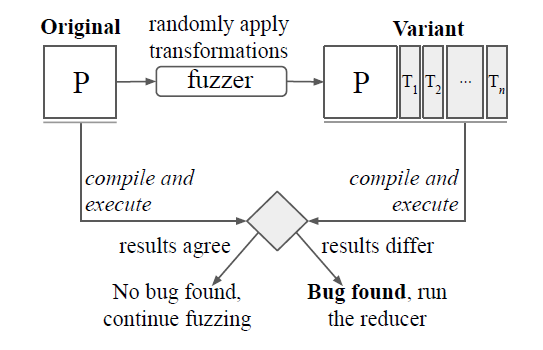
\includegraphics[scale=0.6]{TRNSF.PNG}
            }
        \end{figure}

    \end{frame}

    \notes{It is important to note that we are not performing optimizations on the program.
    We are morphing the program into different forms, which semantically should represent the same program/algorithm.}

    %Give an example.
    \begin{frame}{Example}

        %Paste the example from the paper. 
        \begin{figure}
            \makebox[\textwidth][c]{
                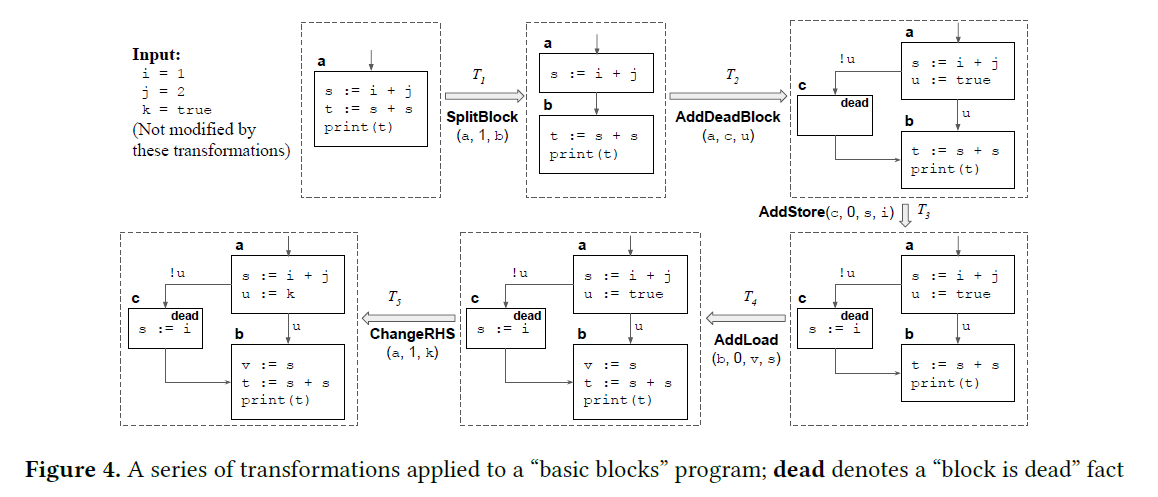
\includegraphics[scale=0.5]{EXAMPLE.PNG}
            }
        \end{figure}

    \end{frame}

    %Explain how we would extract from the example details about bugus.
    \begin{frame}{Example - cnt'd}

        Suppose bug is introduced by adding just a Dead Block and Obfuscating the fact that it is dead. 
        Then the minimal bug (after reduction) would be as below:

        \begin{figure}
            \centering
            \makebox[\textwidth][c]{
                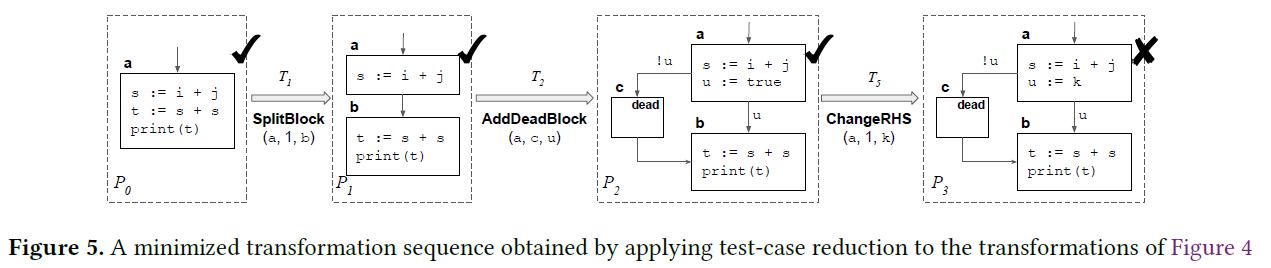
\includegraphics[scale=0.45]{REDUCTION_EX.PNG}
            }
        \end{figure}
        
    \end{frame}

    \notes{Minimal bug set is only w.r.t. the set of transformations we apply. 
    It could be that another set of transformations could reproduce the "same" but and that set being smaller than the previous one.
    But we do not still have a fixed definition of compiler bugs, so it is non-trivial to address.}

    %Explain in layman's terms how the deduplication is done using transformation set. 
    \begin{frame}{Deduplication process}

        Two test exhibiting bugs are the same bug if they are produced using the same set of program transformations (heuristic approach). 
        The algorithm adopted is as follows:
        \begin{figure}
            \centering
            \makebox[\textwidth][c]{
            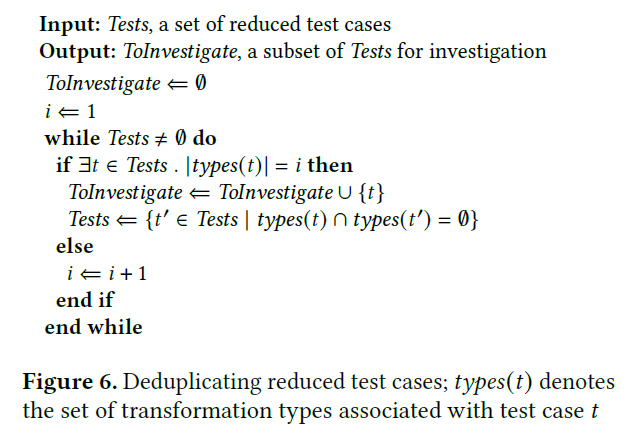
\includegraphics[scale=0.6]{DEDUP-ALGO.PNG}
            }
        \end{figure}

    \end{frame}

    \notes{This is a heuristic approach. 
    It could be that two sets of transformations represent the same bug, but the sets themselves not being the same.
    To prove that unequal sets represent different bugs, we would first need to gather independant transformations.
    This could be a decade worth of work. }

    %Explain in layman's terms how reduction of the test case is done using transformation set. 
    \begin{frame}{Reduction process}
        \begin{enumerate}
            \item Take the sequence of transformations used to induce bugs. 
            \item Test out every subsequence of the transformation.
            \item Can leverage the extra information of facts (preconditions for each transformation).
            \item Will get transformation dependance chains and our search space for reduction would reduce greatly. 
        \end{enumerate}    

        %Refer to the example above and show them how certain transformation sets form a dependant chain. 
    
    \end{frame}

    \notes{We could model this problem using the theory of graphs.
    I think minimal coloring of graph would better help us choose transformations which are not dependant. 
    Have they used this approach? 
    I am unsure.}
    
    %TODO still
    \begin{frame}{SpirvFuzz}

        Takes three arguments - 
        \begin{enumerate}
            \item SPIR-V module.
            \item Input on which the module will execute.
            \item Set of types of transformations.
        \end{enumerate}

        Tool features upto 85 transformations. Some of them are:
        \begin{enumerate}
            \item \textit{CompositeConstruct}
            \item \textit{ReplaceConstWithUniform}
            \item \textit{AddFunction}
            \item \textit{MoveBlockDown}
        \end{enumerate}
    
    \end{frame}

    \notes{SPIR-V module is what is used by Vulkan type libraries.}

    %Miscompilation detection examples 

    \begin{frame}{Miscompilation Bug Example 1}
        
        %Place the figure here of the compilation bug in Mesa
        \begin{figure}
            \makebox[\textwidth][c]{
                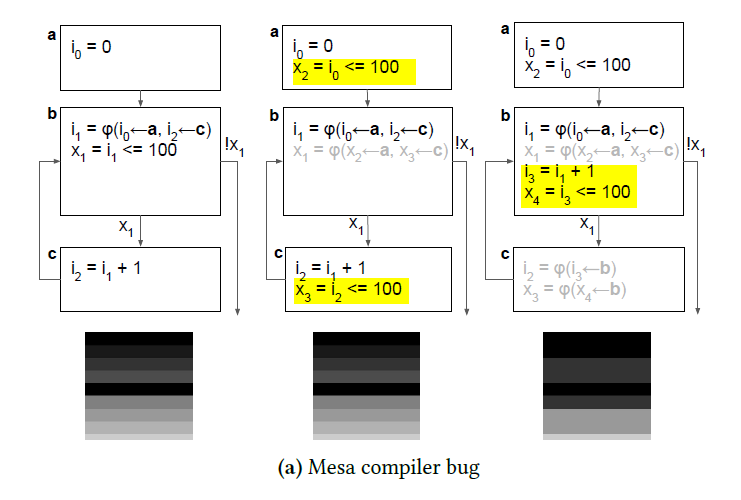
\includegraphics[scale=0.7]{MESA-BUG.PNG}
            }
        \end{figure}

    \end{frame}

    \notes{The bug exists only because for some reason the last iteration of the loop is not performed.
    It is interesting to observe that even though in the example the loop iterations are fixed, the program after compilation fails to loop those fixed amount of times.
    This surely hints towards a bug being in the optimization phase. 
    However, I do not have enough expertise on this.
    Perhaps the interested one can go check the bug report and how they fixed it in the compiler.}

    \begin{frame}{Miscompilation Bug Example 2}

        %Place figure here of the compilation bug in Pixel 5
        \begin{figure}
            \makebox[\textwidth][c]{
                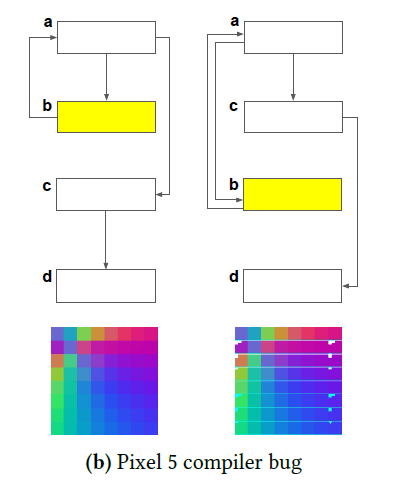
\includegraphics[scale=0.7]{PIXEL5-BUG.PNG}
            }
        \end{figure}

    \end{frame}

    \notes{The bug introduced was just by shifting code around, basically reordering independant instructions.
    It is still interesting that a bug could exist.
    Which I most likely attribute to the optimization phase.}

    %Effectiveness w.r.t existing tools
    \begin{frame}{Comparison with glsl-fuzz}

        \begin{enumerate}
            \item Bug Finding Ability.
            \item Quality of Test-Case reduction.
            \item Effectiveness of Test-Case deduplication.
        \end{enumerate}

    \end{frame}

    \notes{The effectiveness in all three spectrums exist, but a theoretical guarantee must exist.
    These tests were performed on a very specific test bed of programs. 
    The difference is not major. 
    For instance, it would be more beneficial to prove that Test Case reduction of SPIR-V Fuzz is guaranteed to give you lesser LOC.
    And the heuristic approach of Deduplication is guaranteed to identify at least the same amount of duplicates as that of glsl-fuzz.
    Perhaps these are future interesting questions to address.}


    \begin{frame}{Thank you}
        Questions?
    \end{frame}

\end{document}